\section{Техническое задание}
\subsection{Основание для разработки}

Полное наименование системы: «База данных агентства недвижимости».
Основанием для разработки программы является приказ ректора ЮЗГУ
от «17» апреля 2025 г. №1828-с «О направлении (допуске) на практику».

\subsection{Цель и назначение разработки}

Программно-информационная система предназначена для создания договоров аренды и договоров купли-продажи в агентстве недвижимости. С системой должны работать следующие группы пользователей:
\begin{itemize}
\item	сотрудник агентства недвижимости;

\item руководство агентства недвижимости.
\end{itemize}
Сотрудник должен иметь возможность добавлять, удалять и редак- тировать клиентов и объекты недвижимости. Руководство агентства недвижимости должно иметь те же возможности, что и сотрудник, а также добавлять и удалять данные сотрудников.

Данная разработка направлена на оптимизацию деятельности агентства      недвижимости.

В рамках этой разработки предусмотрены следующие задачи:
\begin{itemize}
\item	создание структуры базы данных;

\item	разработка дизайна пользовательского интерфейса;

\item	разработка методов отображения данных из базы данных;

\item	разработка инструментов для администрирования базы данных, чтобы поддерживать актуальность информации.
\end{itemize}

\subsection{Требования к программной системе}

\subsubsection{Требования к данным}

Входными данными для системы являются:
\begin{itemize}
\item	информация о сотруднике, предоставляемая им в процессе реги- страции в системе;

\item	информация о покупателе, предоставляемая им в процессе оформ- ления сделки;

\item	информация о владельце объекта недвижимости, предоставляемая им в процессе регистрации в системе;

\item	информация об объекте недвижимости.
\end{itemize}
Выходными данными для системы являются:
\begin{itemize}
\item	список сотрудников;

\item	список клиентов;

\item	список объектов недвижимости;

\item	созданный договор аренды ;

\item	созданный договор купли-продажи;

\item	сообщения об ошибках.
\end{itemize}

\subsubsection{Функциональные требования}

Приложение имеет две группы пользователей с разными правами: руководство и сотрудники.

Сотрудникам должны быть доступны следующие функции:
\begin{itemize}
\item	добавление покупателей;

\item	добавление владельцев недвижимости;

\item	добавление объектов недвижимости;

\item	просмотр информации о сотрудниках;

\item	просмотр информации о покупателях;

\item	просмотр информации о владельцах объектов недвижимости;

\item	просмотр информации о объектах недвижимости;

\item	удаление  различной информации;

\item	создание договоров аренды;

\item	создание договоров купли-продажи;

\item	удаление договоров.
\end{itemize}
На рисунке ~\ref{user_precedent_diagram:image} изображены прецеденты для сотрудника агентства.

\begin{figure}[H]
	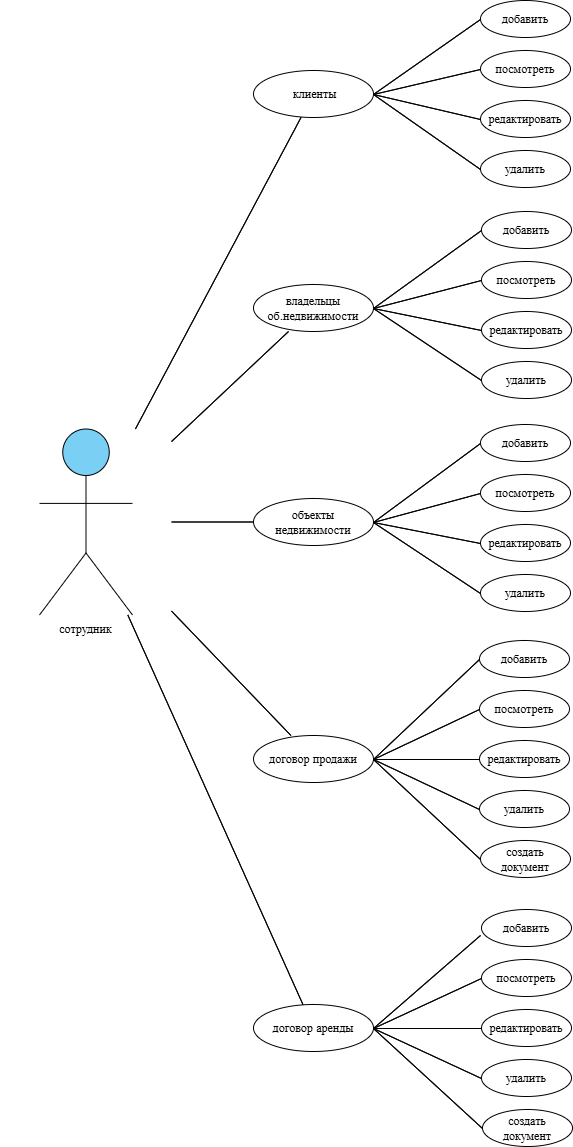
\includegraphics[width=0.73\linewidth]{диаграм_сотрудник}
	\caption{Прецеденты для сотрудника}
	\label{user_precedent_diagram:image}
\end{figure}

Руководству должны быть доступны следующие функции:
\begin{itemize}
\item	добавление сотрудников;

\item	удаление сотрудников;

\item	добавление покупателей;

\item	добавление владельцев недвижимости;

\item	добавление объектов недвижимости;

\item	просмотр информации о сотрудниках;

\item	просмотр информации о покупателях;

\item	просмотр информации о владельцах объектов недвижимости;

\item	просмотр информации о объектах недвижимости;

\item	удаление  различной информации;

\item	создание договоров аренды;

\item	создание договоров купли-продажи;

\item	удаление договоров.
\end{itemize}
\paragraph{Сценарий прецедента сотрудника «добавление информации о покупателе/арендаторе»}

Основной успешный сценарий для прецедента «добавление информации о покупателе/арендаторе».
\begin{enumerate}
\item	Открыть окно «добавить покупателя/арендатора».

\item	Заполнить данные покупателя/арендатора.

\item	Нажать кнопку «добавить»
\end{enumerate}
\paragraph{Сценарий прецедента сотрудника «просмотр информации о покупателе/арендаторе»}

Основной успешный сценарий для прецедента «просмотр информации о покупателе/арендаторе».
\begin{enumerate}
\item	Открыть окно «посмотреть покупателей/арендаторов».
\end{enumerate}
\paragraph{Сценарий прецедента сотрудника «добавление информации о продавце/арендодателе»}

Основной успешный сценарий для прецедента «добавление информации о продавце/арендодателе».
\begin{enumerate}
\item	Открыть окно «добавить продавца/арендодателя».

\item	Заполнить данные продавца/арендодателя.

\item	Нажать кнопку «добавить».
\end{enumerate}
\paragraph{Сценарий прецедента сотрудника «просмотр информации о продавце/арендодателе»}

Основной успешный сценарий для прецедента «просмотр информации о продавце/арендодателе».
\begin{enumerate}
\item Открыть окно «посмотреть продавца/арендодателя».
\end{enumerate}
\paragraph{Сценарий прецедента сотрудника «добавление объекта недвижимости»}

Основной успешный сценарий для прецедента «добавление объекта недвижимости».
\begin{enumerate}
\item	Открыть окно «добавить объект недвижимости».

\item	Заполнить информацию об объекте недвижимости.

\item	Нажать кнопку «добавить»
\end{enumerate}
\paragraph{Сценарий прецедента сотрудника «просмотр объектов недвижимости»}

Основной успешный сценарий для прецедента «просмотр объектов недвижимости».
\begin{enumerate}
\item	Открыть окно «просмотреть объекты недвижимости».
\end{enumerate}
\paragraph{Сценарий прецедента сотрудника «добавить договор купли/продажи»}

Основной успешный сценарий для прецедента «добавить договор купли/продажи».
\begin{enumerate}
\item	Открыть окно «добавить договор купли/продажи».

\item	Заполнить все данные.

\item	Нажать кнопку «добавить».
\end{enumerate}
\paragraph{Сценарий прецедента сотрудника «посмотреть договора купли/продажи»}

Основной успешный сценарий для прецедента «посмотреть договор купли/продажи».
\begin{enumerate}
\item	Открыть окно «посмотреть договор купли/продажи».

\item	Выбрать договор.

\item	Нажать кнопку «создать договор».

\item	Сохранить договор на устройстве.
\end{enumerate}
\paragraph{Сценарий прецедента сотрудника «добавить договор аренды»}

Основной успешный сценарий для прецедента «добавить договор аренды».
\begin{enumerate}
\item	Открыть окно «добавить договор аренды».

\item	Заполнить все данные.

\item	Нажать кнопку «добавить».
\end{enumerate}
\paragraph{Сценарий прецедента сотрудника «посмотреть договор аренды»}

Основной успешный сценарий для прецедента «просмотреть договора аренды».
\begin{enumerate}
\item	Открыть окно «посмотреть договор аренды».

\item	Выбрать договор.

\item	Нажать кнопку «создать договор».

\item	Сохранить договор на устройстве.
\end{enumerate}
\paragraph{Сценарий прецедента руководителя «Добавление сотрудника»}

Основной успешный сценарий для прецедента «Добавление сотрудника».
\begin{enumerate}
\item	Открыть окно «добавить сотрудника».

\item	Заполнить данные сотрудника.

\item	Нажать кнопку «добавить».
\end{enumerate}
\paragraph{Сценарий прецедента руководителя «Просмотр сотрудников»}

Основной успешный сценарий для прецедента «Просмотр сотрудников».
\begin{enumerate}
\item	Открыть окно «просмотреть сотрудников агентства».
\end{enumerate}

\subsubsection{Требования пользователя к интерфейсу приложения}

Приложение должно иметь следующие окна:
\begin{itemize}
\item	Главное окно;

\item	Окно с добавлением покупателя/арендатора;

\item	Окно с просмотром покупателей/арендаторов;

\item	Окно с добавлением продавцов/арендодателей;

\item	Окно с просмотром продавцов/арендодателей;

\item	Окно с добавлением объектов недвижимости;

\item	Окно с просмотром объектов недвижимости;

\item	Окно с добавлением сотрудников;

\item	Окно с просмотром сотрудников;

\item	Окно с добавлением договоров продажи;

\item	Окно с просмотром договоров продажи;

\item	Окно с добавлением договоров аренды;

\item	Окно с просмотром договоров аренды.
\end{itemize}
\clearpage

На рисунке ~\ref{gl_okno:image} представлен интерфейс приложения.

\begin{figure}[H]
	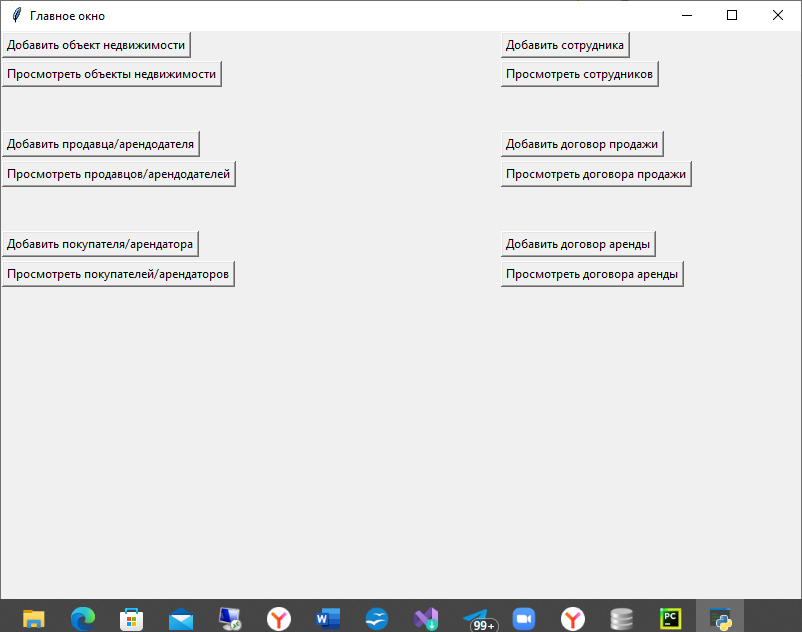
\includegraphics[width=1\linewidth]{главн_окно}
	\caption{Интерфейс приложения}
	\label{gl_okno:image}
\end{figure}


\subsubsection{Нефункциональные требования}

\paragraph{Требования к безопасности}

Необходимо устранить уязвимости, возможные для приложений:
\begin{itemize}
\item роли пользователей: Установить разные роли (администратор, агент, клиент) с соответствующими правами доступа;

\item защита от атак с перебором паролей: Внедрить блокировку учетной записи после нескольких неудачных попыток входа;

\item шифрование данных: Использовать алгоритмы шифрования для хранения конфиденциальных данных, таких как пароли и личная информация;

\item защита передачи данных: Все данные, передаваемые по сети, должны быть защищены с помощью HTTPS;

\item защита от SQL-инъекций: Использовать технологии ORM (Object-Relational Mapping) и параметризованные запросы для защиты от SQL-инъекций;

\item ведение журналов: Реализовать механизмы ведения журналов действий пользователей и администраторов для последующего анализа;

\item управление доступом к данным: Ограничить доступ пользователей к конфиденциальной информации (например, информации о других пользователях, сделках);

\item регулярные обновления: Обеспечить своевременное обновление всех библиотек и зависимостей для защиты от известных уязвимостей;

\item безопасность сервера: Хранить серверы в защищенных помещениях с ограниченным доступом;

\item резервное копирование: Регулярно делать резервные копии базы данных и важных данных;

\item обучение сотрудников: Проводить тренинги по вопросам безопасности для пользователей и сотрудников агентства;

\item соблюдение законодательства: Соблюдать местное и международное законодательство по защите персональных данных (такие как GDPR).
\end{itemize}
\paragraph{Требования к программному обеспечению}

Для создания программного решения потребуется подготовить ряд ключевых элементов: 
\begin{itemize}
\item фреймворк Laravel, обеспечивающий структуру и упрощающий разработку; 

\item среду исполнения Python, необходимую для запуска кода;

\item систему управления базами данных.
\end{itemize}
Laravel демонстрирует широкую совместимость, работая на актуальных операционных системах, таких как Windows, macOS и Linux.

\paragraph{Требования к аппаратному обеспечению}

Для работы приложения требуется дисковое пространство не менее 1 Гб. Рекомендуется использовать процессор c 2 или более ядрами и частотой 2 ГГц или выше.

\subsection{Требования к оформлению документации}

Стадии разработки программного обеспечения и требования к программной документации для вычислительной техники, комплексов и систем любого назначения и области применения регламентируются ГОСТ 19.102–77. В состав программной документации входят:
\begin{itemize}
\item	анализ предметной области;

\item	техническое задание;

\item	технический проект;

\item	рабочий проект.
\end{itemize}